%%%%%%%%%%%%%%%%%%%%%%%%%%%%%%%%%%%%%%%%%%%%%%%%%%%%%%%%%%%
%\section{Example cases}
%%%%%%%%%%%%%%%%%%%%%%%%%%%%%%%%%%%%%%%%%%%%%%%%%%%%%%%%%%%
%
%
%%%%%%%%%%%%%%%%%%%%%%%%%%%%%%%%%%%%%%%%%%%%%%%%%%%%%%%%%%%
\subsection{Descendant fix: proxies (a)}
%%%%%%%%%%%%%%%%%%%%%%%%%%%%%%%%%%%%%%%%%%%%%%%%%%%%%%%%%%%
%
%
\begin{frame}[t, negative]
	\subsectionpage
\end{frame}
%
%
\begin{frame}
	{Proxies (a)\footnote{\citet{McElreath_2020}, chapter 11 (p. 340); \citet{McElreath_2022}, lecture 10}}
	%
	\begin{columns}
		%
		\begin{column}{0.5\textwidth}
			%
			research question, 
			%
			\begin{itemize}
				%
				\item \textcolor{blue}{Does $X$ has a (direct) effect on $M$?}
				%
			\end{itemize}
			
			variables,
			%
			\begin{itemize}
				%
				\item X, teacher experience
				\item E, instruction quality (old, new) \\
				{\small (unobserved)}
				\item A, proxy variable (e.g. age)
				\item M, teachers' score in mathematics \\
				{\small (from a standardized evaluation)}
				%
			\end{itemize}
			%
		\end{column}
		%
		\begin{column}{0.5\textwidth}  
			%
			\begin{equ}
				%
				M = \left\{ \begin{aligned} 
					A \leftarrow & \; f_{A}(E,U_{A}) \\
					X \leftarrow & \; f_{X}(E,U_{X}) \\
					M \leftarrow & \; f_{M}(E, X, U_{M})\\
					U \sim & \; P(\pmb{U})
				\end{aligned} \right
				%
				\caption*{(a) structural model}
				%
			\end{equ}
			%
			\begin{figure}
				%
				\begin{tikzpicture}
					% nodes
					\node[formula] at (-2,0) {$U_{X}$};
					\node[formula] at (-1,-0.3) {$X$};
					\node[formula] at (0,1) {$E$};
					\node[formula] at (1,1) {$A$};
					\node[formula] at (2,0.75) {$U_{A}$};
					\node[formula] at (1,-0.3) {$M$};
					\node[formula] at (2,0) {$U_{M}$};
					
					% paths
					\draw [{Circle [open]}-{latex}](-1.7,0)--(-1,0); % Ux->X
					\draw [{Circle}-{latex}](-1.03,0)--(0.9,0); % X->L
					\draw [{Circle [open]}-{latex}{Circle}](1.7,0)--(0.9,0); % Um->M
					\draw [-{latex}](0,0.75)--(-0.95,0.05); % E->X
					\draw [{Circle [open]}-{latex}](0,0.8)--(0.9,0.05); % E->M
					\draw [-{latex}](0.1,0.75)--(0.90,0.75); % E->A
					\draw [{Circle [open]}-{latex}{Circle}](1.7,0.75)--(0.9,0.75); % Ul->U2
					
					% extra
					\node at (0,-0.25) {$(?)$}; % symbol
				\end{tikzpicture}
				%
				\caption*{(b) causal diagram}
				%
			\end{figure}
			%
		\end{column}
		%
	\end{columns}
	%
\end{frame}
%
%
\begin{frame}
	{Simulation setting}
	%
	\begin{columns}
		%
		\begin{column}{0.5\textwidth}
			%
			\begin{figure}
				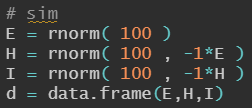
\includegraphics[scale=0.8]{descendant1_code.png}
				\caption*{(c) R code}
			\end{figure}
			%
			\textcolor{blue}{Implications},
			%
			\begin{itemize}
				\item \ndsep{A}{M} \\
				\item \ndsep{A}{X} \\
				\item \dsep{X}{M} \; | E {\small (impossible)}
				\item \dsep{X}{M} \; | A {\small (partially)}
			\end{itemize}
			%
		\end{column}
		%
		\begin{column}{0.5\textwidth}  
			%
			\begin{equ}
				%
				M = \left\{ \begin{aligned} 
					A \leftarrow & \; f_{A}(E,U_{A}) \\
					X \leftarrow & \; f_{X}(E,U_{X}) \\
					M \leftarrow & \; f_{M}(E, X, U_{M})\\
					U \sim & \; P(\pmb{U})
				\end{aligned} \right
				%
				\caption*{(a) structural model}
				%
			\end{equ}
			%
			\begin{figure}
				%
				\begin{tikzpicture}
					% nodes
					\node[formula] at (-2,0) {$U_{X}$};
					\node[formula] at (-1,-0.3) {$X$};
					\node[formula] at (0,1) {$E$};
					\node[formula] at (1,1) {$A$};
					\node[formula] at (2,0.75) {$U_{A}$};
					\node[formula] at (1,-0.3) {$M$};
					\node[formula] at (2,0) {$U_{M}$};
					
					% paths
					\draw [{Circle [open]}-{latex}{Circle}](-1.7,0)--(-0.9,0); % Ux->X
					%\draw [{Circle}-{latex}](-1.03,0)--(0.9,0); % X->M
					\draw [{Circle [open]}-{latex}{Circle}](1.7,0)--(0.9,0); % Um->M
					\draw [-{latex}](0,0.75)--(-0.95,0.05); % E->X
					\draw [{Circle [open]}-{latex}](0,0.8)--(0.9,0.05); % E->M
					\draw [-{latex}](0.1,0.75)--(0.90,0.75); % E->A
					\draw [{Circle [open]}-{latex}{Circle}](1.7,0.75)--(0.9,0.75); % UA->A
				\end{tikzpicture}
				%
				\caption*{(b) causal diagram}
				%
			\end{figure}
			%
		\end{column}
		%
	\end{columns}
	%
\end{frame}
%
%
\begin{lhframe}[rhgraphic={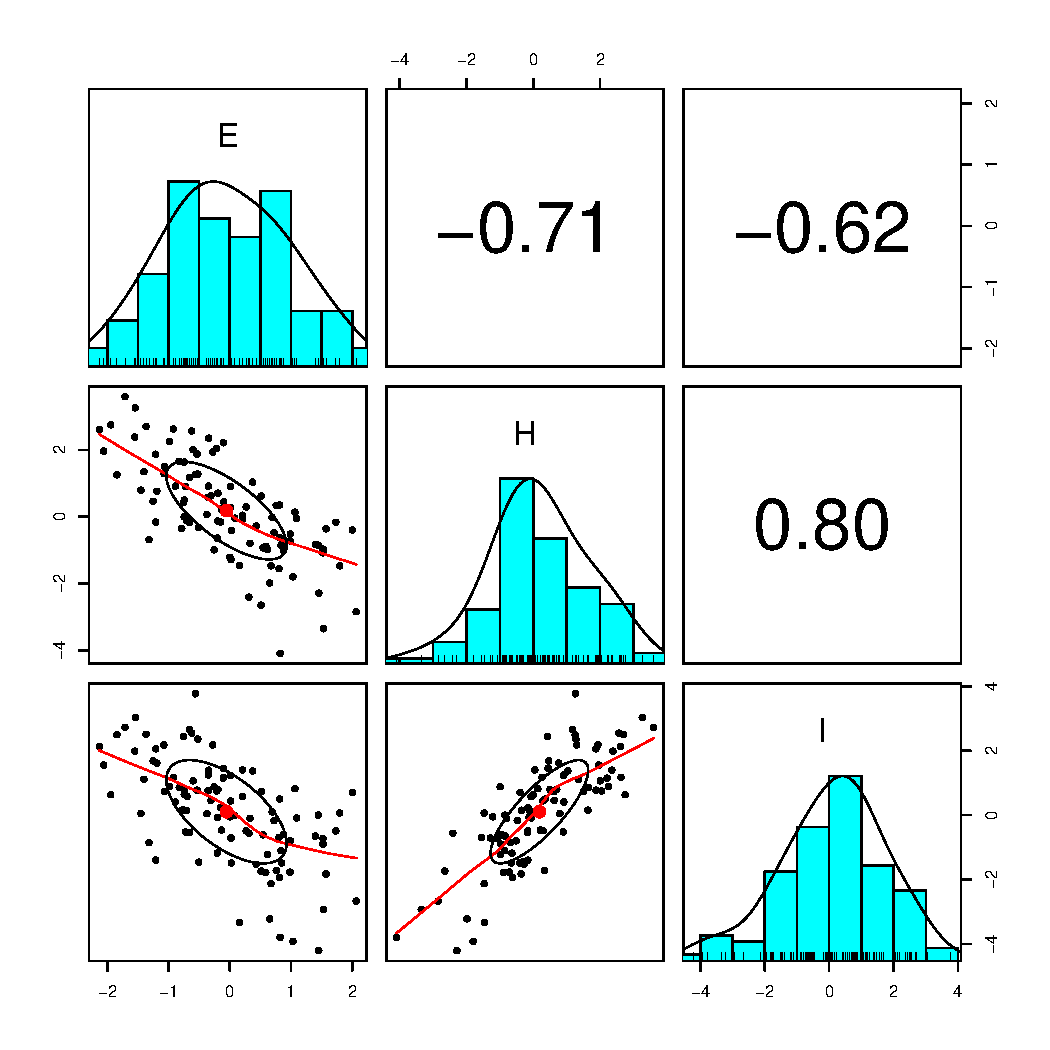
\includegraphics[scale=0.4]{descendant1_panel.pdf}}]
	{``Eyeballing" analysis}
	
	based on \textcolor{blue}{correlation analysis},
	%
	\begin{itemize}
		%
		\item $Cor(A,M)<0$ goes in line with our ``rudimentary" understanding of the data, \\
		{\small (old teachers has old type of instruction, and lower score)}
		%
		\item but $cor(X, M)<0$ does not go in line with our ``understanding"\\
		{\small (the more experienced, the less the score?)}
		%
		\item but we \textcolor{blue}{might include} $Z$ in our statistical model \\
		{\small (based on univariate (linear) correlation)}
		%
	\end{itemize}
	%
\end{lhframe}
%
%
\begin{lhframe}[rhgraphic={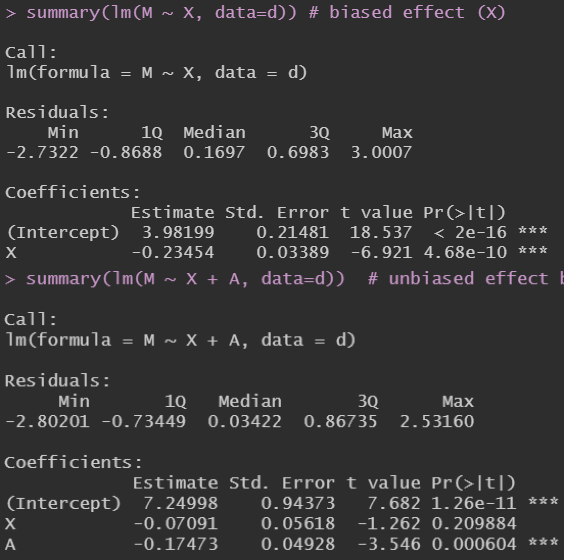
\includegraphics[scale=0.3]{descendant1_reg.png}}]
	{Regression, regression!!}
	
	based on \textcolor{blue}{statistical analysis},
	%
	\begin{itemize}
		%
		\item we now have two models with two different effects
		\item which one is the ``truth"?
		%
	\end{itemize}
	%
\end{lhframe}
%
%
\begin{lhframe}[rhgraphic={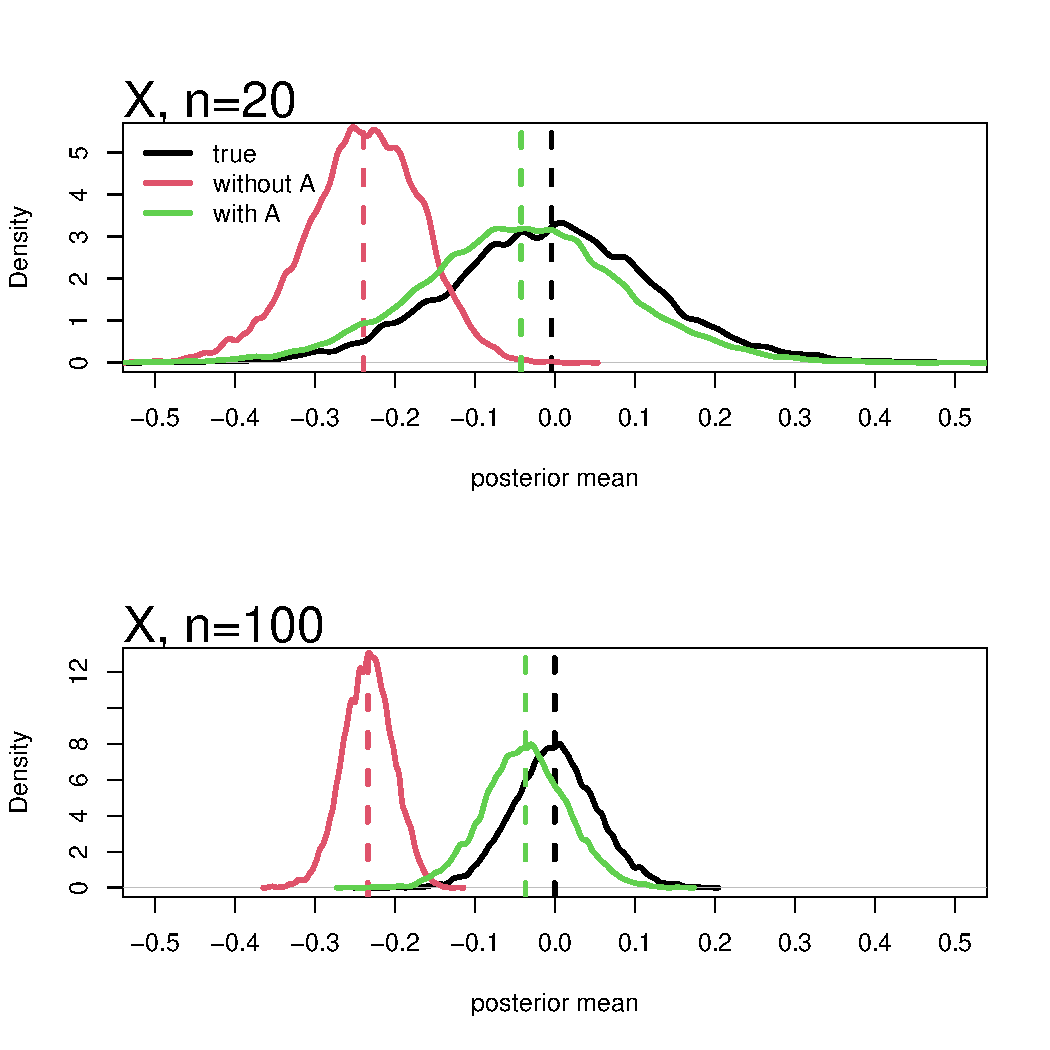
\includegraphics[scale=0.45]{descendant1a_samplesize.pdf}}]
	{The data tell-tell story!!}
	
	imagine we can continue sampling,
	%
	\begin{itemize}
		%
		\item top: $10,000$ samples $n=20$
		\item bottom: $10,000$ samples $n=100$
		%
	\end{itemize}
	
	the larger the sample size,
	%
	\begin{itemize}
		%
		\item under the model \textcolor{blue}{without $A$}, \\
		the more \textcolor{blue}{certain} you are about your \textcolor{blue}{biased} estimates
		%
		\item under the model \textcolor{blue}{with $A$}, \\
		the more \textcolor{blue}{certain} you are about your \textcolor{blue}{less biased} estimates
		%
	\end{itemize}
	%
\end{lhframe}
%
%
\begin{frame}
	{So, what is going on?}
	%
	\begin{columns}
		%
		\begin{column}{0.5\textwidth}
			%
			based on \textcolor{blue}{DAG} and \textcolor{blue}{statistical model},
			%
			\begin{itemize}
				%
				\item stratifying on $A$ \textcolor{blue}{partially blocks} the backdoor path produced by the confounder $E$ \\
				i.e. when stratifying by $A$ you are partially stratifying by $E$
				%
			\end{itemize}
			%
		\end{column}
		%
		\begin{column}{0.5\textwidth}  
			%
			\begin{equ}
				%
				M = \left\{ \begin{aligned} 
					A \leftarrow & \; f_{A}(E,U_{A}) \\
					X \leftarrow & \; f_{X}(E,U_{X}) \\
					M \leftarrow & \; f_{M}(E, X, U_{M})\\
					U \sim & \; P(\pmb{U})
				\end{aligned} \right
				%
				\caption*{(a) structural model}
				%
			\end{equ}
			%
			\begin{figure}
				%
				\begin{tikzpicture}
					% nodes
					\node[formula] at (-2,0) {$U_{X}$};
					\node[formula] at (-1,-0.3) {$X$};
					\node[formula] at (0,1) {$E$};
					\node[formula] at (1,1) {$A$};
					\node[formula] at (2,0.75) {$U_{A}$};
					\node[formula] at (1,-0.3) {$M$};
					\node[formula] at (2,0) {$U_{M}$};
					
					% paths
					\draw [{Circle [open]}-{latex}](-1.7,0)--(-1,0); % Ux->X
					\draw [{Circle}-{latex}](-1.03,0)--(0.9,0); % X->L
					\draw [{Circle [open]}-{latex}{Circle}](1.7,0)--(0.9,0); % Um->M
					\draw [-{latex}](0,0.75)--(-0.95,0.05); % E->X
					\draw [{Circle [open]}-{latex}](0,0.8)--(0.9,0.05); % E->M
					\draw [-{latex}](0.1,0.75)--(0.90,0.75); % E->A
					\draw [{Circle [open]}-{latex}{Circle}](1.7,0.75)--(0.9,0.75); % Ul->U2
					
					% extra
					\node at (0,-0.25) {$(?)$}; % symbol
				\end{tikzpicture}
				%
				\caption*{(b) causal diagram}
				%
			\end{figure}
			%
		\end{column}
		%
	\end{columns}
	%
\end{frame}
%
%
\begin{lhframe}[rhgraphic={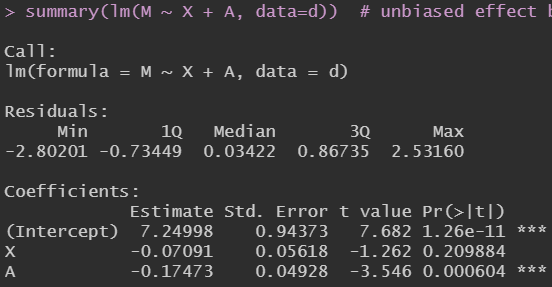
\includegraphics[scale=0.5]{descendant1_reg2.png}}]
	{the dream team!!}
	
	based on \textcolor{blue}{DAG} and \textcolor{blue}{statistical analysis},
	%
	\begin{itemize}
		%
		\item the less biased model is the second, \\
		{\small \textcolor{blue}{(assuming our DAG is true)} }
		%
	\end{itemize}
	%
\end{lhframe}
%
%
\begin{frame}
	{But age cause experience, right?}
	%
	\begin{columns}
		%
		\begin{column}{0.5\textwidth}
			%
			research question, 
			%
			\begin{itemize}
				%
				\item \textcolor{blue}{Does $X$ has a (direct) effect on $M$?}
				%
			\end{itemize}
			
			variables,
			%
			\begin{itemize}
				%
				\item X, teacher experience
				\item E, instruction quality (old, new) \\
				{\small (unobserved)}
				\item A, cause variable (e.g. age)
				\item M, teachers' score in mathematics \\
				{\small (from a standardized evaluation)}
				%
			\end{itemize}
			%
		\end{column}
		%
		\begin{column}{0.5\textwidth}  
			%
			\begin{equ}
				%
				M = \left\{ \begin{aligned} 
					A \leftarrow & \; f_{A}(U_{A}) \\
					X \leftarrow & \; f_{X}(E,U_{X}) \\
					M \leftarrow & \; f_{M}(E, X, U_{M})\\
					U \sim & \; P(\pmb{U})
				\end{aligned} \right
				%
				\caption*{(a) structural model}
				%
			\end{equ}
			%
			\begin{figure}
				%
				\begin{tikzpicture}
					% nodes
					\node[formula] at (-2,0) {$U_{X}$};
					\node[formula] at (-1,-0.3) {$X$};
					\node[formula] at (0,1) {$E$};
					\node[formula] at (1,1) {$A$};
					\node[formula] at (2,0.75) {$U_{A}$};
					\node[formula] at (1,-0.3) {$M$};
					\node[formula] at (2,0) {$U_{M}$};
					
					% paths
					\draw [{Circle [open]}-{latex}](-1.7,0)--(-1,0); % Ux->X
					\draw [{Circle}-{latex}](-1.03,0)--(0.9,0); % X->L
					\draw [{Circle [open]}-{latex}{Circle}](1.7,0)--(0.9,0); % Um->M
					\draw [-{latex}](0,0.75)--(-0.95,0.05); % E->X
					\draw [{Circle [open]}-{latex}](0,0.8)--(0.9,0.05); % E->M
					\draw [-{latex}](0.90,0.75)--(0.1,0.75); % A->E
					\draw [{Circle [open]}-{latex}{Circle}](1.7,0.75)--(0.9,0.75); % Ul->U2
					
					% extra
					\node at (0,-0.25) {$(?)$}; % symbol
				\end{tikzpicture}
				%
				\caption*{(b) causal diagram}
				%
			\end{figure}
			%
		\end{column}
		%
	\end{columns}
	%
\end{frame}
%
%
\begin{lhframe}[rhgraphic={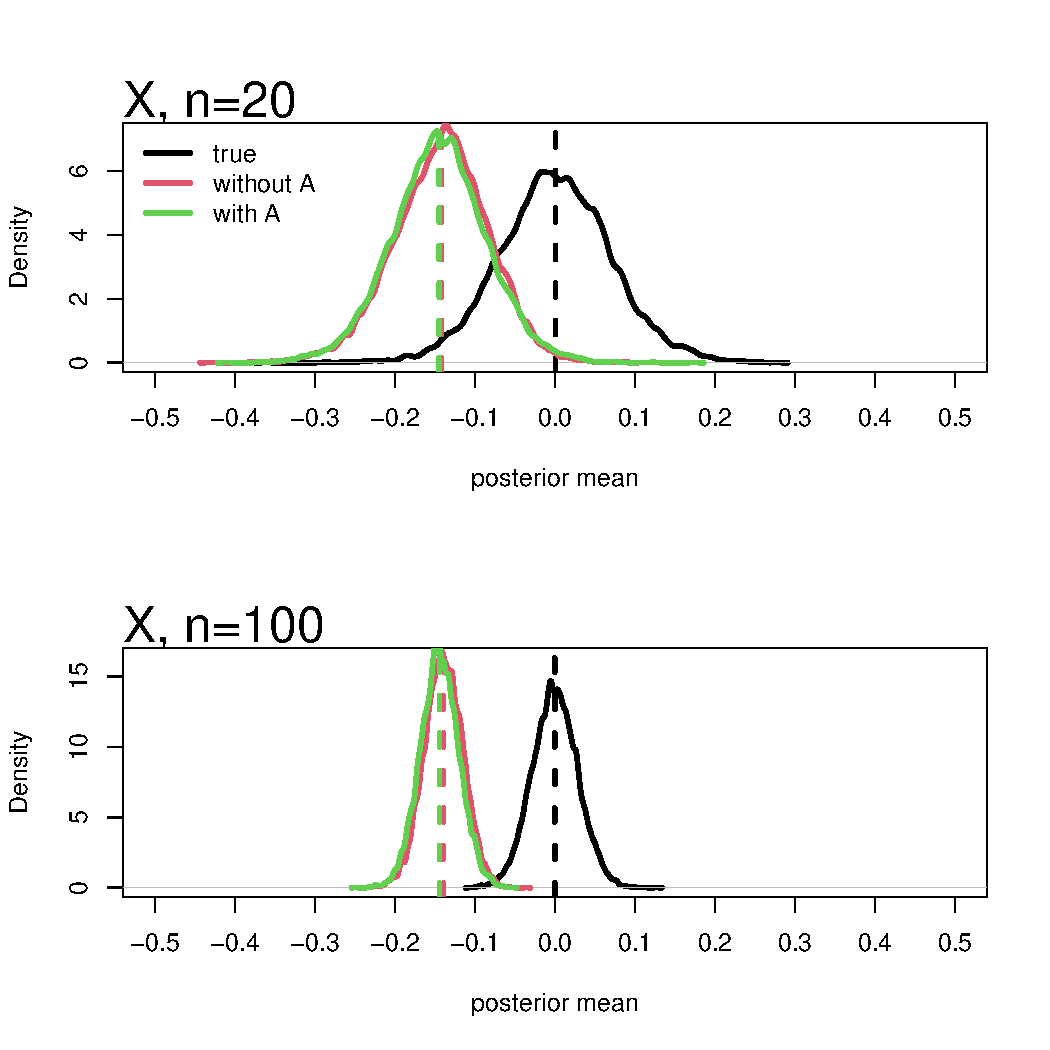
\includegraphics[scale=0.45]{descendant1b_samplesize.pdf}}]
	{But age cause experience, right?}
	
	imagine we can continue sampling,
	%
	\begin{itemize}
		%
		\item top: $10,000$ samples $n=20$
		\item bottom: $10,000$ samples $n=100$
		%
	\end{itemize}
	
	the larger the sample size,
	%
	\begin{itemize}
		%
		\item under any model including $A$, \\
		the more \textcolor{blue}{certain} you are about your \textcolor{blue}{biased} estimates
		%
	\end{itemize}
	%
\end{lhframe}
%
%
%%%%%%%%%%%%%%%%%%%%%%%%%%%%%%%%%%%%%%%%%%%%%%%%%%%%%%%%%%%
\subsection{Descendant fix: proxies (b)}
%%%%%%%%%%%%%%%%%%%%%%%%%%%%%%%%%%%%%%%%%%%%%%%%%%%%%%%%%%%
%
%
\begin{frame}[t, negative]
	\subsectionpage
\end{frame}
%
%
\begin{frame}
	{Proxies (b)\footnote{\citet{McElreath_2020}, chapter 11 (p. 340); \citet{McElreath_2022}, lecture 10}}
	%
	\begin{columns}
		%
		\begin{column}{0.5\textwidth}
			%
			research question, 
			%
			\begin{itemize}
				%
				\item \textcolor{blue}{Do females are discriminated in school admissions, i.e. does $G \rightarrow A$?}
				%
			\end{itemize}
			
			variables,
			%
			\begin{itemize}
				%
				\item G, gender
				\item D, department of application
				\item A, admission
				\item $U_{X}$, confound (e.g. ability) \\
				{\small (unobserved)}
				\item $T_{i}$, test scores, with $i=1,2,3$ \\
				{\small ($U_{Ti}$ are reliabilities)}
				%
			\end{itemize}
			%
		\end{column}
		%
		\begin{column}{0.5\textwidth}  
			%
			\begin{equ}
				%
				M = \left\{ \begin{aligned} 
					G \leftarrow & \; f_{G}(U_{G}) \\
					D \leftarrow & \; f_{D}(G,U_{X},U_{D}) \\
					A \leftarrow & \; f_{A}(D, G,U_{X},U_{A}) \\
					T_{i} \leftarrow & \; f_{T}(U_{X},U_{Ti}) \\
					U \sim & \; P(\pmb{U})
				\end{aligned} \right
				%
				\caption*{(a) structural model}
				%
			\end{equ}
			%
			\begin{figure}
				%
				\begin{tikzpicture}
					% nodes
					\node[formula] at (-2,0) {$U_{G}$};
					\node[formula] at (-1,-0.3) {$G$};
					\node[formula] at (-1,1) {$U_{D}$};
					\node[formula] at (0,1) {$D$};
					\node[formula] at (0.8,1) {$U_{X}$};
					\node[formula] at (2,-0.3) {$U_{A}$};
					\node[formula] at (1,-0.3) {$A$};
					\node[formula] at (2,0.3) {$T_{1}$};
					\node[formula] at (2,0.75) {$T_{2}$};
					\node[formula] at (2,1.2) {$T_{3}$};
					
					% paths
					\draw [{Circle [open]}-{latex}{Circle}](-1.7,0)--(-0.9,0); % Ug->G
					\draw [-{latex}](-0.9,0)--(0.9,0); % G->A
					\draw [{Circle [open]}-{latex}{Circle}](2,0)--(0.9,0); % Ua->A
					\draw [-{latex}](-0.95,0.05)--(0,0.75); % G->D
					\draw [{Circle [color=red]}-{latex}](0,0.8)--(0.9,0.1); % D->A
					\draw [{Circle[open]}-{latex}](-1,0.75)--(0,0.75); % Ud->D
					\draw [-{latex}](0.90,0.75)--(0.1,0.75); % Ux->D
					\draw [{Circle[open]}-{latex}](0.95,0.8)--(0.95,0.05); % Ux->A
					\draw [-{latex}{Circle}](1,0.75)--(1.7,0.3); % Ux->T1
					\draw [-{latex}{Circle}](1,0.75)--(1.7,0.75); % Ux->T2
					\draw [-{latex}{Circle}](1,0.75)--(1.7,1.2); % Ux->T3
					
					% extra
					\node at (0,-0.25) {$(?)$}; % symbol
				\end{tikzpicture}
				%
				\caption*{(b) causal diagram}
				%
			\end{figure}
			%
		\end{column}
		%
	\end{columns}
	%
\end{frame}
%
%
\begin{frame}
	{Simulation setting}
	%
	\begin{columns}
		%
		\begin{column}{0.5\textwidth}
			%
			\begin{figure}
				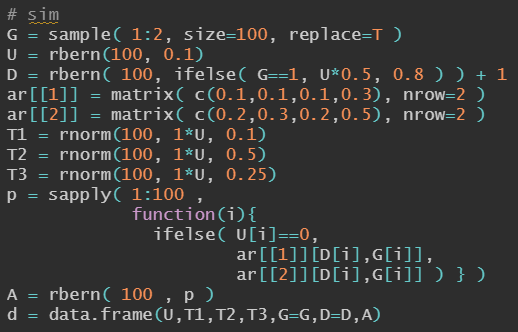
\includegraphics[scale=0.7]{descendant2_code.png}
				\caption*{(c) R code}
			\end{figure}
			%
		\end{column}
		%
		\begin{column}{0.5\textwidth}  
			%
			\begin{equ}
				%
				M = \left\{ \begin{aligned} 
					G \leftarrow & \; f_{G}(U_{G}) \\
					D \leftarrow & \; f_{D}(G,U_{X},U_{D}) \\
					A \leftarrow & \; f_{A}(D, G,U_{X},U_{A}) \\
					T_{i} \leftarrow & \; f_{T}(U_{X},U_{T}) \\
					U \sim & \; P(\pmb{U})
				\end{aligned} \right
				%
				\caption*{(a) structural model}
				%
			\end{equ}
			%
			\begin{figure}
				%
				\begin{tikzpicture}
					% nodes
					\node[formula] at (-2,0) {$U_{G}$};
					\node[formula] at (-1,-0.3) {$G$};
					\node[formula] at (-1,1) {$U_{D}$};
					\node[formula] at (0,1) {$D$};
					\node[formula] at (0.8,1) {$U_{X}$};
					\node[formula] at (2,-0.3) {$U_{A}$};
					\node[formula] at (1,-0.3) {$A$};
					\node[formula] at (2,0.3) {$T_{1}$};
					\node[formula] at (2,0.75) {$T_{2}$};
					\node[formula] at (2,1.2) {$T_{3}$};
					
					% paths
					\draw [{Circle [open]}-{latex}{Circle}](-1.7,0)--(-0.9,0); % Ug->G
					\draw [-{latex}](-0.9,0)--(0.9,0); % G->A
					\draw [{Circle [open]}-{latex}{Circle}](2,0)--(0.9,0); % Ua->A
					\draw [-{latex}](-0.95,0.05)--(0,0.75); % G->D
					\draw [{Circle [color=red]}-{latex}](0,0.8)--(0.9,0.1); % D->A
					\draw [{Circle[open]}-{latex}](-1,0.75)--(0,0.75); % Ud->D
					\draw [-{latex}](0.90,0.75)--(0.1,0.75); % Ux->D
					\draw [{Circle[open]}-{latex}](0.95,0.8)--(0.95,0.05); % Ux->A
					\draw [-{latex}{Circle}](1,0.75)--(1.7,0.3); % Ux->T1
					\draw [-{latex}{Circle}](1,0.75)--(1.7,0.75); % Ux->T2
					\draw [-{latex}{Circle}](1,0.75)--(1.7,1.2); % Ux->T3
					
					% extra
					\node at (0,-0.25) {$(?)$}; % symbol
				\end{tikzpicture}
				%
				\caption*{(b) causal diagram}
				%
			\end{figure}
			%
		\end{column}
		%
	\end{columns}
	%
\end{frame}
%
%
\begin{lhframe}[rhgraphic={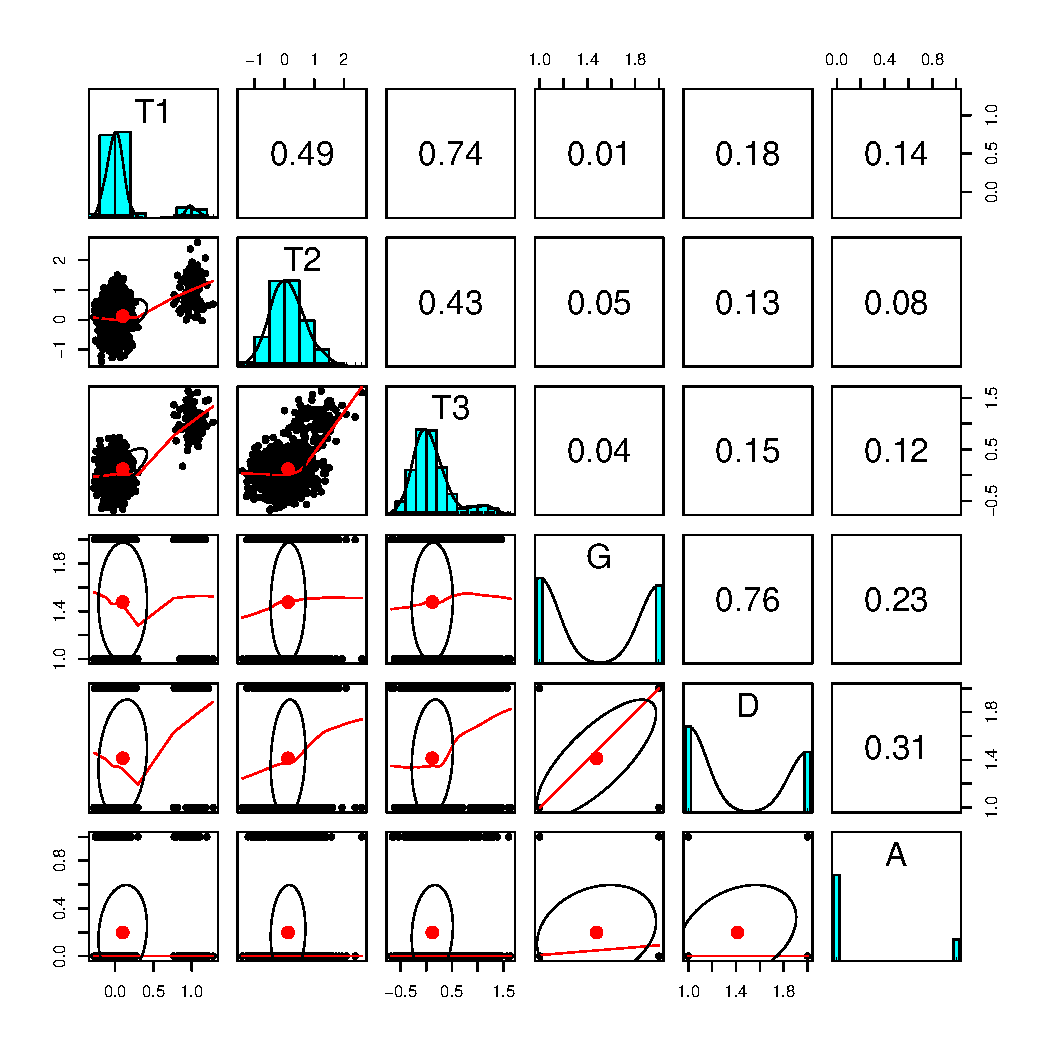
\includegraphics[scale=0.4]{descendant2_panel.pdf}}]
	{``Eyeballing" analysis}
	
	based on \textcolor{blue}{correlation analysis},
	%
	\begin{itemize}
		%
		\item the task has become more complex \\
		{\small (more variables to decide on)}
		%
		\item while $cor(H, I)>0$ indicate the more you work the more you gain \\
		{\small (but is it the only way?)}
		%
		\item since $cor(H, I)$ is high we \textcolor{blue}{might include it} as a covariate in our statistical model \\
		{\small (to improve the precision?)}
		%
	\end{itemize}
	%
\end{lhframe}
%
%
\begin{lhframe}[rhgraphic={\includegraphics[scale=0.3]{descendant2_reg.png}}]
	{Regression, regression!!}
	
	based on \textcolor{blue}{statistical analysis},
	%
	\begin{itemize}
		%
		\item we now have two models with two different ``levels" of effects
		\item which one is the ``truth"?
		%
	\end{itemize}
	%
\end{lhframe}
%
%
\begin{lhframe}[rhgraphic={\includegraphics[scale=0.45]{descendant2_samplesize.pdf}}]
	{The data tell-tell story!!}
	
	imagine we can continue sampling,
	%
	\begin{itemize}
		%
		\item top: $10,000$ samples $n=20$
		\item bottom: $10,000$ samples $n=100$
		%
	\end{itemize}
	
	under the \textcolor{blue}{incorrect model},\\
	the larger the sample size,
	%
	\begin{itemize}
		%
		\item the more \textcolor{blue}{certain} you are about your \textcolor{blue}{biased} estimates
		%
	\end{itemize}
	%
\end{lhframe}
%
%
\begin{frame}
	{So, what is going on?}
	%
	\begin{columns}
		%
		\begin{column}{0.5\textwidth}
			%
			based on \textcolor{blue}{DAG} and \textcolor{blue}{statistical model},
			%
			\begin{itemize}
				%
				\item stratifying on $I$ explains variability in $H$ (is his descendant) \\
				remaining variance is explained by $E$ \\
				{\small (big chunk is already explained)}
				%
				\item but there is more!!: \\
				$H$ is now a collider in the path $E \rightarrow H \leftarrow U_{H}$ \textcolor{blue}{(virtual collider)}, \\
				then, stratifying by $I$ \textcolor{blue}{opens that path} (biasing the estimates).
				%
			\end{itemize}
			%
		\end{column}
		%
		\begin{column}{0.5\textwidth}  
			%
			\begin{equ}
				%
				M = \left\{ \begin{aligned} 
					E \leftarrow & \; f_{E}(U_{E}) \\
					H \leftarrow & \; f_{H}(E,U_{H}) \\
					I \leftarrow & \; f_{I}(H,U_{I}) \\
					U \sim & \; P(\pmb{U})
				\end{aligned} \right
				%
				\caption*{(a) structural model}
				%
			\end{equ}
			%
			\begin{figure}
				%
				\begin{tikzpicture}
					% nodes
					\node[formula] at (-2,0) {$U_{E}$};
					\node[formula] at (-1,-0.3) {$E$};
					\node[formula] at (1,1.5) {$U_{I}$};
					\node[formula] at (0,1) {$I$};
					\node[formula] at (2,0) {$U_{H}$};
					\node[formula] at (1,-0.3) {$H$};
					
					% paths
					\draw [{Circle [open]}-{latex}{Circle}](-1.7,0)--(-0.9,0); % Ue->E
					\draw [-{latex}](-0.9,0)--(0.9,0); % E->H
					\draw [{Circle [open]}-{latex}{Circle}](1.7,0)--(0.9,0); % Uh->H
					\draw [-{latex}{Circle}](0.95,0.05)--(0,0.8); % H->I
					\draw [{Circle [open]}-{latex}](0.9,1.3)--(0.1,0.8); % Ui->I
					
					% extra
					\node at (0,-0.25) {$(?)$}; % symbol
				\end{tikzpicture}
				%
				\caption*{(b) causal diagram}
				%
			\end{figure}
			%
		\end{column}
		%
	\end{columns}
	%
\end{frame}
%
%
\begin{lhframe}[rhgraphic={\includegraphics[scale=0.5]{descendant2_reg1.png}}]
	{the dream team!!}
	
	based on \textcolor{blue}{DAG} and \textcolor{blue}{statistical analysis},
	%
	\begin{itemize}
		%
		\item the less biased model is the first, \\
		{\small \textcolor{blue}{(assuming our DAG is true)} }
		%
	\end{itemize}
	%
\end{lhframe}
%
%
%%%%%%%%%%%%%%%%%%%%%%%%%%%%%%%%%%%%%%%%%%%%%%%%%%%%%%%%%%%
\subsection{Descendant bias: case control}
%%%%%%%%%%%%%%%%%%%%%%%%%%%%%%%%%%%%%%%%%%%%%%%%%%%%%%%%%%%
%
%
\begin{frame}[t, negative]
	\subsectionpage
\end{frame}
%
%
\begin{frame}
	{Case control\footnote{\citet{McElreath_2022}, lecture 6; \citet{Cinelli_et_al_2021} (p. 8, 19), \citet{Hernan_2020}, lesson 3}}
	%
	\begin{columns}
		%
		\begin{column}{0.5\textwidth}
			%
			also, 
			%
			\begin{itemize}
				%
				\item \textcolor{blue}{virtual collider}
				\item an instance of descendant bias
				%
			\end{itemize}
			
			research question, 
			%
			\begin{itemize}
				%
				\item \textcolor{blue}{Does $E$ has a (direct) effect on $H$?}
				\item Should we include $I$ on our model?
				%
			\end{itemize}
			
			variables,
			%
			\begin{itemize}
				%
				\item E, education 
				\item H, hours in occupation \\
				{\small (standardized)}
				\item I, income
				%
			\end{itemize}
			%
		\end{column}
		%
		\begin{column}{0.5\textwidth}  
			%
			\begin{equ}
				%
				M = \left\{ \begin{aligned} 
					E \leftarrow & \; f_{E}(U_{E}) \\
					H \leftarrow & \; f_{H}(E,U_{H}) \\
					I \leftarrow & \; f_{I}(H,U_{I}) \\
					U \sim & \; P(\pmb{U})
				\end{aligned} \right
				%
				\caption*{(a) structural model}
				%
			\end{equ}
			%
			\begin{figure}
				%
				\begin{tikzpicture}
					% nodes
					\node[formula] at (-2,0) {$U_{E}$};
					\node[formula] at (-1,-0.3) {$E$};
					\node[formula] at (1,1.5) {$U_{I}$};
					\node[formula] at (0,1) {$I$};
					\node[formula] at (2,0) {$U_{H}$};
					\node[formula] at (1,-0.3) {$H$};
					
					% paths
					\draw [{Circle [open]}-{latex}{Circle}](-1.7,0)--(-0.9,0); % Ue->E
					\draw [-{latex}](-0.9,0)--(0.9,0); % E->H
					\draw [{Circle [open]}-{latex}{Circle}](1.7,0)--(0.9,0); % Uh->H
					\draw [-{latex}{Circle}](0.95,0.05)--(0,0.8); % H->I
					\draw [{Circle [open]}-{latex}](0.9,1.3)--(0.1,0.8); % Ui->I
					
					% extra
					\node at (0,-0.25) {$(?)$}; % symbol
				\end{tikzpicture}
				%
				\caption*{(b) causal diagram}
				%
			\end{figure}
			%
		\end{column}
		%
	\end{columns}
	%
\end{frame}
%
%
\begin{frame}
	{Simulation setting}
	%
	\begin{columns}
		%
		\begin{column}{0.5\textwidth}
			%
			\begin{figure}
				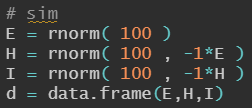
\includegraphics[scale=0.8]{descendant3_code.png}
				\caption*{(c) R code}
			\end{figure}
			%
			\textcolor{blue}{Implications},
			%
			\begin{itemize}
				\item \ndsep{E}{H} \\
				\item \dsep{E}{I} \; | H
				\item \ndsep{E}{$U_{H}$} \; | I \\
				{\small \textcolor{blue}{(virtual collider)} }
			\end{itemize}
			%
		\end{column}
		%
		\begin{column}{0.5\textwidth}  
			%
			\begin{equ}
				%
				M = \left\{ \begin{aligned} 
					E \leftarrow & \; f_{E}(U_{E}) \\
					H \leftarrow & \; f_{H}(E,U_{H}) \\
					I \leftarrow & \; f_{I}(H,U_{I}) \\
					U \sim & \; P(\pmb{U})
				\end{aligned} \right
				%
				\caption*{(a) structural model}
				%
			\end{equ}
			%
			\begin{figure}
				%
				\begin{tikzpicture}
					% nodes
					\node[formula] at (-2,0) {$U_{E}$};
					\node[formula] at (-1,-0.3) {$E$};
					\node[formula] at (1,1.5) {$U_{I}$};
					\node[formula] at (0,1) {$I$};
					\node[formula] at (2,0) {$U_{H}$};
					\node[formula] at (1,-0.3) {$H$};
					
					% paths
					\draw [{Circle [open]}-{latex}{Circle}](-1.7,0)--(-0.9,0); % Ue->E
					\draw [-{latex}](-0.9,0)--(0.9,0); % E->H
					\draw [{Circle [open]}-{latex}{Circle}](1.7,0)--(0.9,0); % Uh->H
					\draw [-{latex}{Circle}](0.95,0.05)--(0,0.8); % H->I
					\draw [{Circle [open]}-{latex}](0.9,1.3)--(0.1,0.8); % Ui->I
				\end{tikzpicture}
				%
				\caption*{(b) causal diagram}
				%
			\end{figure}
			%
		\end{column}
		%
	\end{columns}
	%
\end{frame}
%
%
\begin{lhframe}[rhgraphic={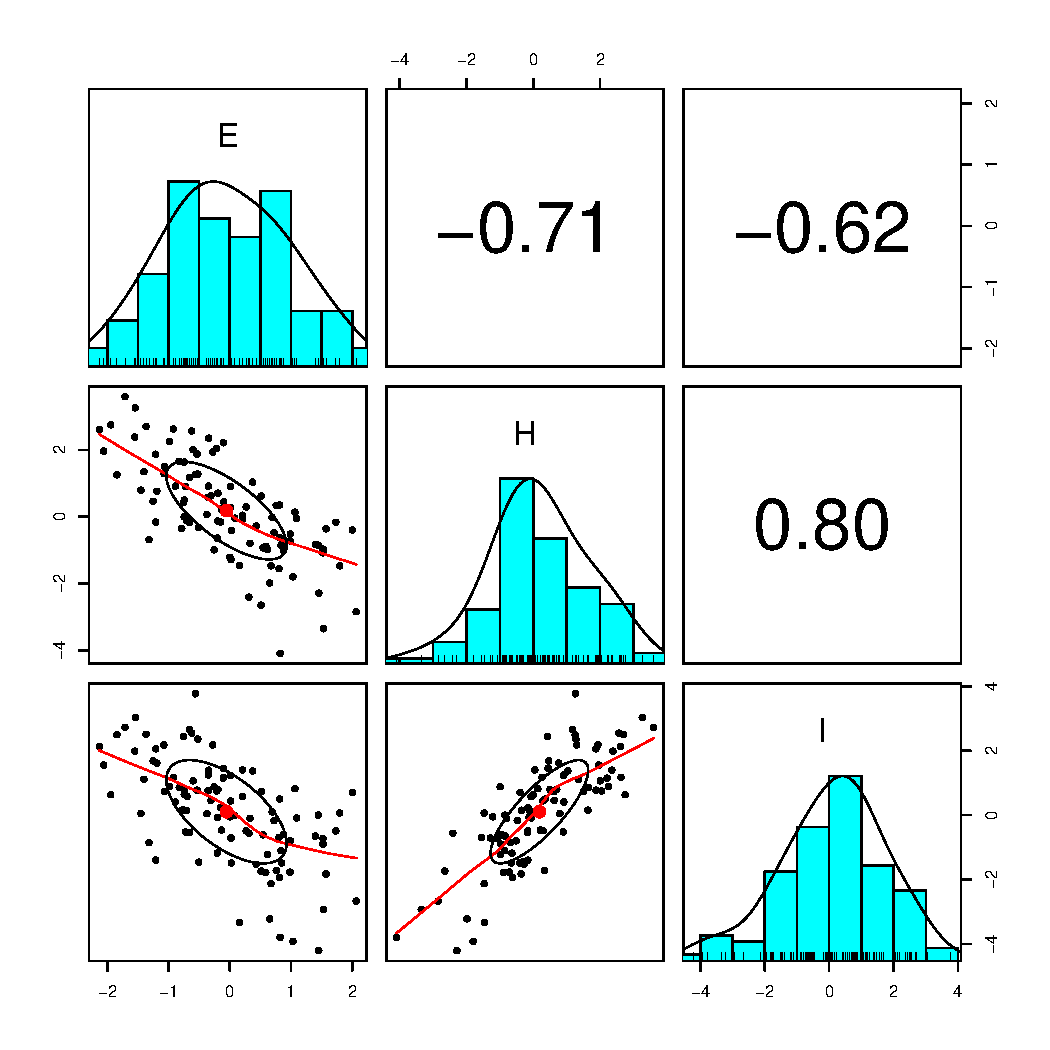
\includegraphics[scale=0.4]{descendant3_panel.pdf}}]
	{``Eyeballing" analysis}
	
	based on \textcolor{blue}{correlation analysis},
	%
	\begin{itemize}
		%
		\item $cor(E, I)<0$ does NOT goes in line of our ``rudimentary" understanding of the data.
		%
		\item while $cor(H, I)>0$ indicate the more you work the more you gain \\
		{\small (but is it the only way?)}
		%
		\item since $cor(H, I)$ is high we \textcolor{blue}{might include it} as a covariate in our statistical model \\
		{\small (to improve the precision?)}
		%
	\end{itemize}
	%
\end{lhframe}
%
%
\begin{lhframe}[rhgraphic={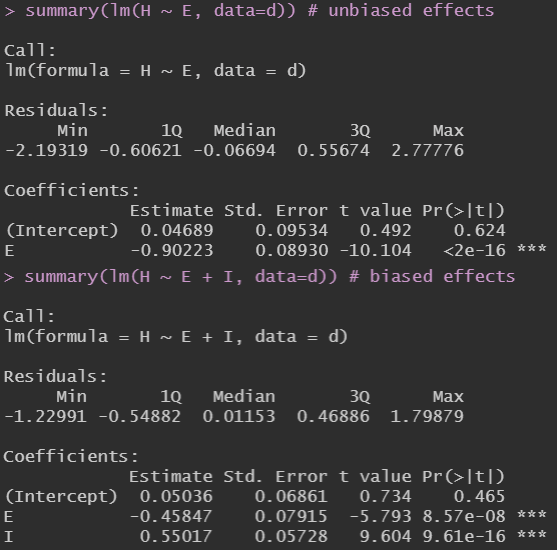
\includegraphics[scale=0.3]{descendant3_reg.png}}]
	{Regression, regression!!}
	
	based on \textcolor{blue}{statistical analysis},
	%
	\begin{itemize}
		%
		\item we now have two models with two different ``levels" of effects
		\item which one is the ``truth"?
		%
	\end{itemize}
	%
\end{lhframe}
%
%
\begin{lhframe}[rhgraphic={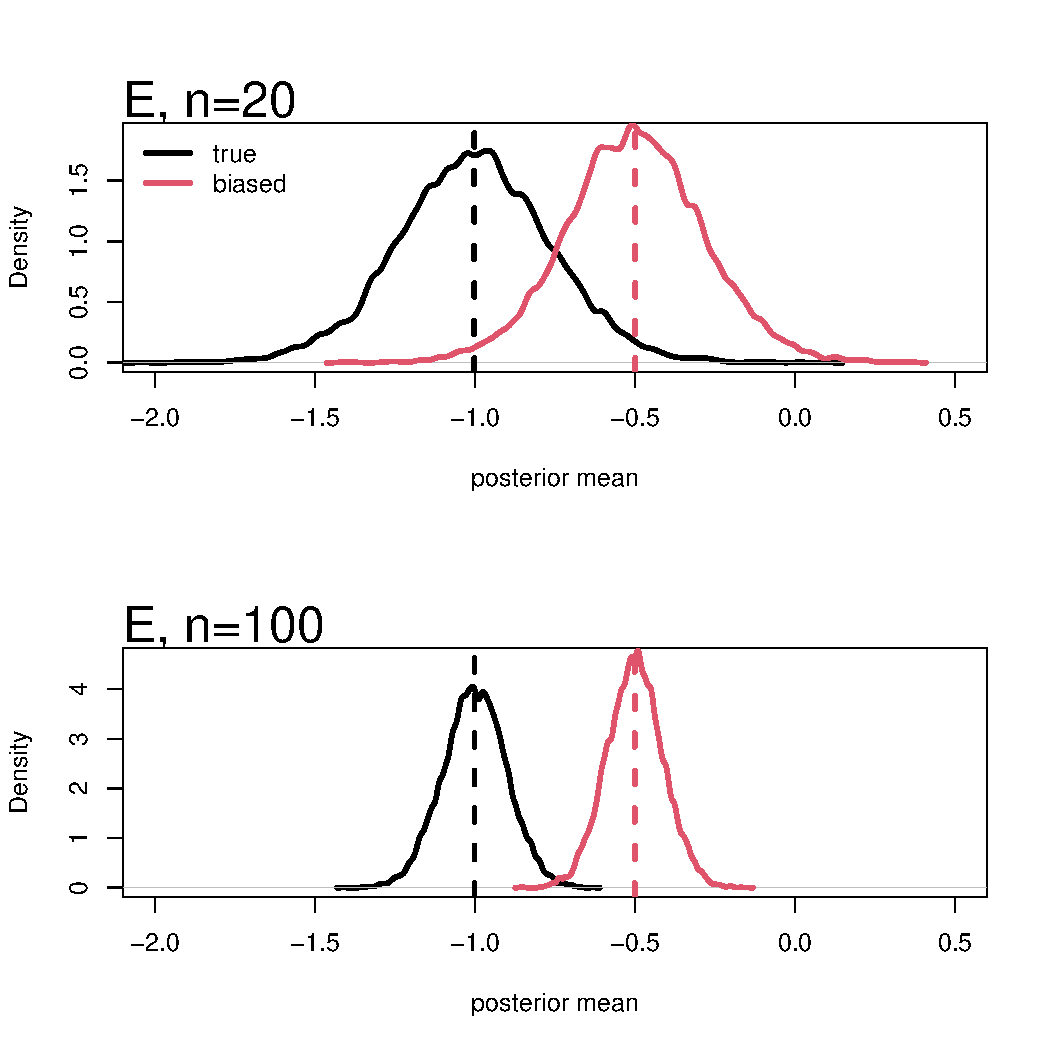
\includegraphics[scale=0.45]{descendant3_samplesize.pdf}}]
	{The data tell-tell story!!}
	
	imagine we can continue sampling,
	%
	\begin{itemize}
		%
		\item top: $10,000$ samples $n=20$
		\item bottom: $10,000$ samples $n=100$
		%
	\end{itemize}
	
	under the \textcolor{blue}{incorrect model},\\
	the larger the sample size,
	%
	\begin{itemize}
		%
		\item the more \textcolor{blue}{certain} you are about your \textcolor{blue}{biased} estimates
		%
	\end{itemize}
	%
\end{lhframe}
%
%
\begin{frame}
	{So, what is going on?}
	%
	\begin{columns}
		%
		\begin{column}{0.5\textwidth}
			%
			based on \textcolor{blue}{DAG} and \textcolor{blue}{statistical model},
			%
			\begin{itemize}
				%
				\item stratifying on $I$ explains variability in $H$ (is his descendant) \\
				remaining variance is explained by $E$ \\
				{\small (big chunk is already explained)}
				%
				\item but there is more!!: \\
				$H$ is now a collider in the path $E \rightarrow H \leftarrow U_{H}$ \textcolor{blue}{(virtual collider)}, \\
				then, stratifying by $I$ \textcolor{blue}{opens that path} (biasing the estimates).
				%
			\end{itemize}
			%
		\end{column}
		%
		\begin{column}{0.5\textwidth}  
			%
			\begin{equ}
				%
				M = \left\{ \begin{aligned} 
					E \leftarrow & \; f_{E}(U_{E}) \\
					H \leftarrow & \; f_{H}(E,U_{H}) \\
					I \leftarrow & \; f_{I}(H,U_{I}) \\
					U \sim & \; P(\pmb{U})
				\end{aligned} \right
				%
				\caption*{(a) structural model}
				%
			\end{equ}
			%
			\begin{figure}
				%
				\begin{tikzpicture}
					% nodes
					\node[formula] at (-2,0) {$U_{E}$};
					\node[formula] at (-1,-0.3) {$E$};
					\node[formula] at (1,1.5) {$U_{I}$};
					\node[formula] at (0,1) {$I$};
					\node[formula] at (2,0) {$U_{H}$};
					\node[formula] at (1,-0.3) {$H$};
					
					% paths
					\draw [{Circle [open]}-{latex}{Circle}](-1.7,0)--(-0.9,0); % Ue->E
					\draw [-{latex}](-0.9,0)--(0.9,0); % E->H
					\draw [{Circle [open]}-{latex}{Circle}](1.7,0)--(0.9,0); % Uh->H
					\draw [-{latex}{Circle}](0.95,0.05)--(0,0.8); % H->I
					\draw [{Circle [open]}-{latex}](0.9,1.3)--(0.1,0.8); % Ui->I
					
					% extra
					\node at (0,-0.25) {$(?)$}; % symbol
				\end{tikzpicture}
				%
				\caption*{(b) causal diagram}
				%
			\end{figure}
			%
		\end{column}
		%
	\end{columns}
	%
\end{frame}
%
%
\begin{lhframe}[rhgraphic={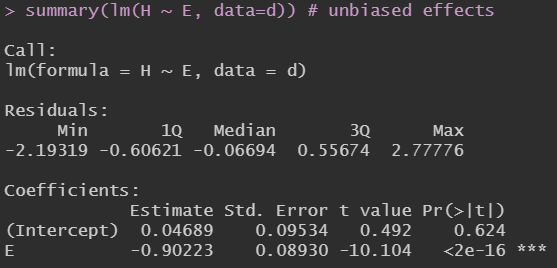
\includegraphics[scale=0.5]{descendant3_reg1.png}}]
	{the dream team!!}
	
	based on \textcolor{blue}{DAG} and \textcolor{blue}{statistical analysis},
	%
	\begin{itemize}
		%
		\item the less biased model is the first, \\
		{\small \textcolor{blue}{(assuming our DAG is true)} }
		%
	\end{itemize}
	%
\end{lhframe}
%
%
\begin{frame}
	{Similar, but different\footnote{\citet{Cinelli_et_al_2021} (p. 7)}}
	%
	\begin{columns}
		%
		\begin{column}{0.5\textwidth}
			%
			research question, 
			%
			\begin{itemize}
				%
				\item \textcolor{blue}{What is the effect of $X$ on $Y$?}
				\item Should we include $Z$ in the model?
				%
			\end{itemize}
			
			variables,
			%
			\begin{itemize}
				%
				\item Z, ``child" of X
				\item X, exposure
				\item Y, outcome
				%
			\end{itemize}
			%
		\end{column}
		%
		\begin{column}{0.5\textwidth}  
			%
			\begin{equ}
				%
				M = \left\{ \begin{aligned} 
					X \leftarrow & \; f_{X}(U_{X}) \\
					Z \leftarrow & \; f_{Z}(X, U_{Z}) \\
					Y \leftarrow & \; f_{Y}(X, U_{Y}) \\
					U \sim & \; P(\pmb{U})
				\end{aligned} \right
				%
				\caption*{(a) structural model}
				%
			\end{equ}
			%
			\begin{figure}
				%
				\begin{tikzpicture}
					% nodes
					\node[formula] at (-2,0.8) {$U_{Z}$};
					\node[formula] at (-1,1) {$Z$};
					\node[formula] at (-2,0) {$U_{X}$};
					\node[formula] at (-1,-0.3) {$X$};
					\node[formula] at (1,-0.3) {$Y$};
					\node[formula] at (2,0) {$U_{Y}$};
					
					% paths
					\draw [{Circle [open]}-{latex}{Circle}](-1.7,0.75)--(-0.9,0.75); % Uz->Z
					\draw [-{latex}](-0.95,0.05)--(-0.95,0.70); % X->Z
					\draw [{Circle [open]}-{latex}{Circle}](-1.7,0)--(-0.9,0); % Ux->X
					\draw [-{latex}](-0.9,0)--(0.9,0); % X->Y
					\draw [{Circle [open]}-{latex}{Circle}](1.7,0)--(0.9,0); % Uy->Y
					
					% extra
					\node at (0,-0.25) {$(?)$}; % symbol
				\end{tikzpicture}
				%
				\caption*{(b) causal diagram}
				%
			\end{figure}
			%
		\end{column}
		%
	\end{columns}
	%
\end{frame}
%
%
\begin{lhframe}[rhgraphic={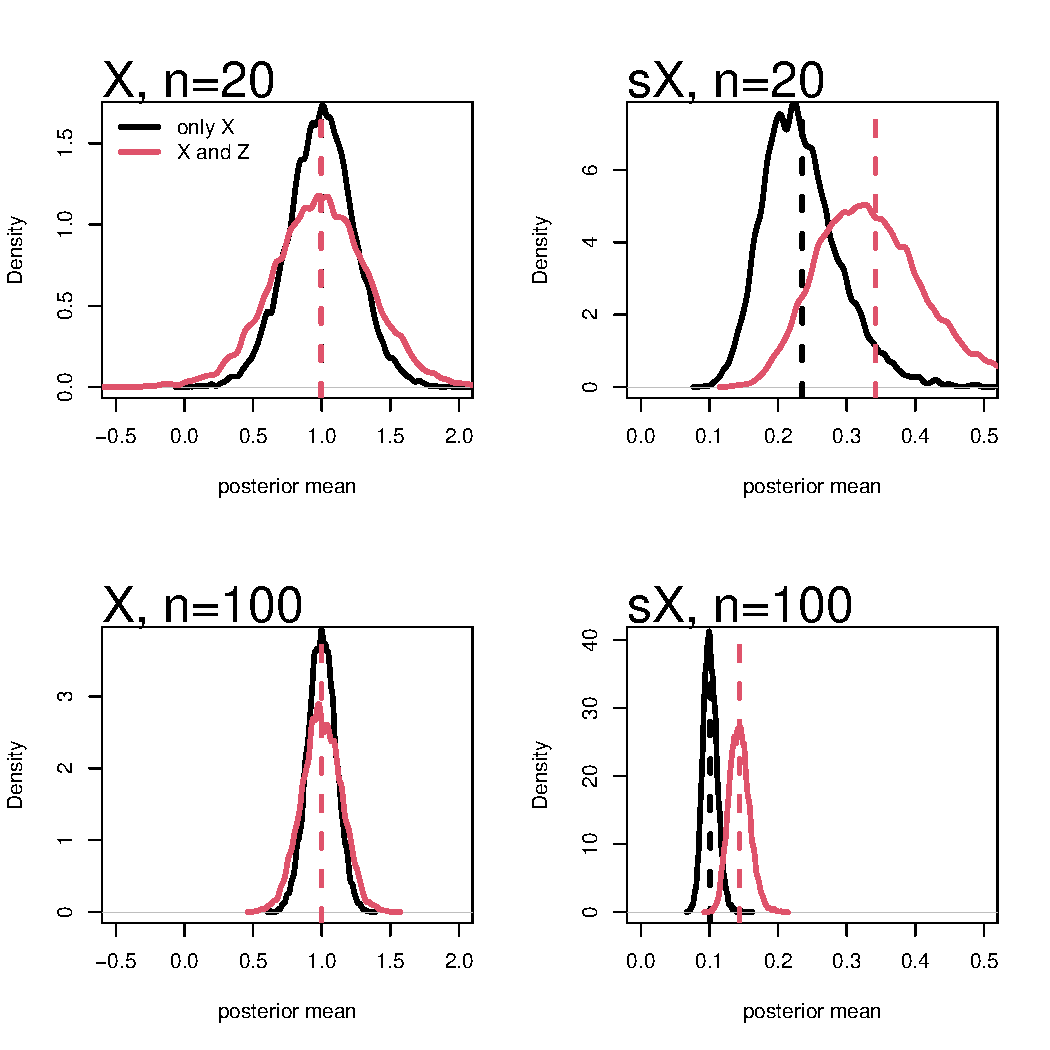
\includegraphics[scale=0.45]{descendant3b_samplesize.pdf}}]
	{Similar, but different}
	
	imagine we can continue sampling,
	%
	\begin{itemize}
		%
		\item top: $10,000$ samples $n=20$
		\item bottom: $10,000$ samples $n=100$
		%
	\end{itemize}
	
	under the \textcolor{blue}{incorrect model},\\
	the larger the sample size,
	%
	\begin{itemize}
		%
		\item you loose \textcolor{blue}{certainty} in your \textcolor{blue}{non-biased} estimates
		%
	\end{itemize}
	%
\end{lhframe}
%
%
